\chapter{Le Montréal 3V2}
\label{montreal}

Nous allons ici présenter la solution sur laquelle nous nous appuyons pour réaliser notre propre radiogoniomètre à effet Doppler, le Montréal 3V2.
Pour réaliser cette documentation nous nous sommes appuyés sur la documentation trouvée sur le site f1lvt \cite{montreal}

\section{Évolution du Montréal}

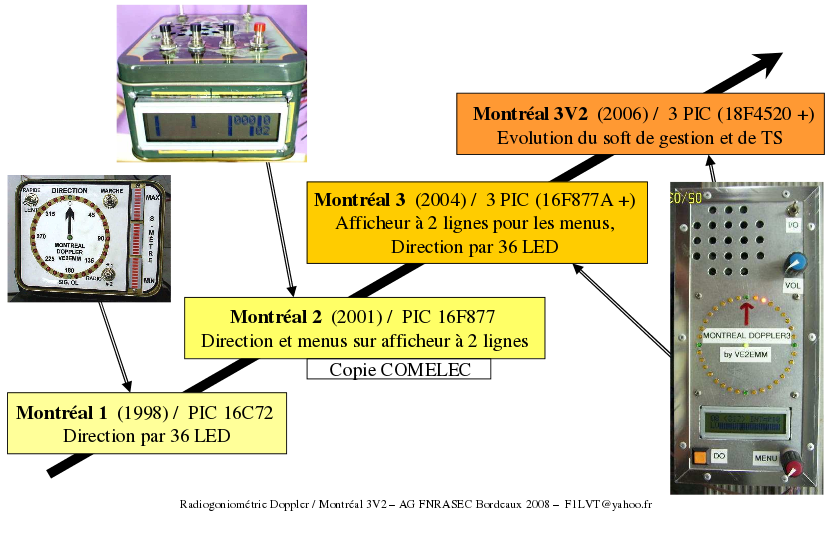
\includegraphics[width=\textwidth]{evolution}
\captionof{figure}{Evolution du Montréal}

\section{Avantages du Montréal 3v2}

\begin{center}
  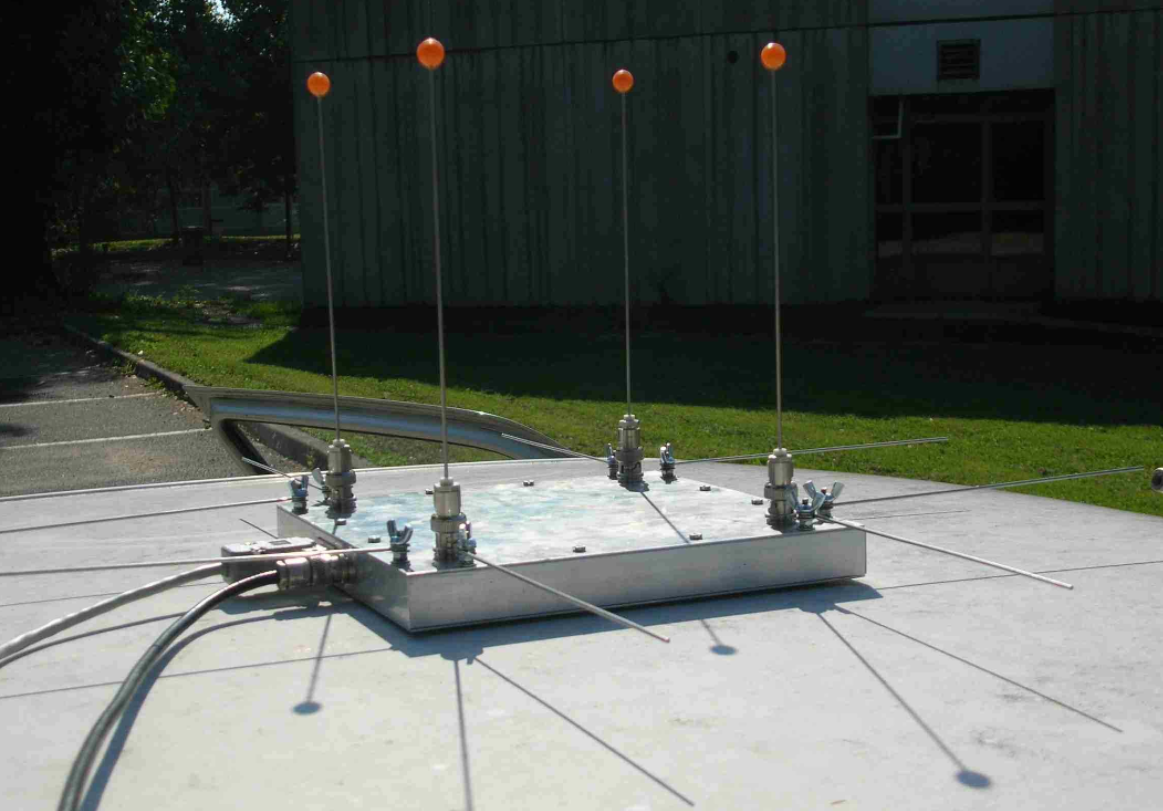
\includegraphics[width=0.5\textwidth]{montreal}
  \captionof{figure}{Photographie prise du Montréal 3v2}
\end{center}

\parindent=15pt
Le Montréal 3v2 sert principalement à l'FNRASEC\footnote{Fédération Nationale des Radioamateurs au service de la Sécurité Civile, agrée de sécurité civile} et aux chasseurs d'onde amateurs. Ce radiogoniomètre est utilisé pour la détection de balise de détresse de 406MHz.

%Parmi ses avantages, on peut noter qu'il est facile à construire, son prix , et il est simple d'utilisation. 

Un des intérêts majeurs du Montréal 3-V2, c'est sa capacité de localiser des signaux très courts, son prix de revient est très raisonnable,son traitement très rapide et la mise en mémoire automatique du dernier relevé. On peut aussi noter qu'il est simple d'utilisation grâce à son affichage à 36 LEDs disposées en cercle et qui indiquent la direction. De plus une LED centrale indique le fonctionnement; verte la direction affichée est bonne, rouge le signal est insuffisant, la direction reste alors figée dans la dernière bonne direction reçue.

%on peut noter son affichage à 36 LED qui indique la direction de manière clair et efficace, et un réglage facilité par son écran LCD ou encore son filtre à capa commutée à très faible largeur de bande (0,5 Hz).

\section{Caractéristiques}

Le Montréal 3v2 est un radiogoniomètre à effet Doppler, il possède donc toutes les caractéristiques associés à ce type de radiogoniomètre.
~\\

\begin{tabular}{ l l l}
Fréquences & distance & moyenne portée\\
 & gamme & 50MHz-1.3GHz\\
 & démodulation & FM\\
Affichage & LED & 36LEDs\\
& écran & LCD en 2 lignes\\
Filtre & capa & très faible largeur de bande (0.5Hz)\\
Coût & & estimé à 50\euro \\
\end{tabular}


\section{Fonctionnement}
La partie centrale contient les circuits d'amplification et de commutation. Les 4 brins verticaux (les brins actifs) se fixent par BNC.

Les antennes sont alimentées de façon séquentielle pour imiter une antenne en rotation. Une fois que les antennes ont capté les ondes provenant du drone, il faut faire une démodulation et enlever tous les bruits.


Un système à LED permet de visualiser la composante continue qui passe dans les antennes. A partir du boîtier Doppler et de son menu de test, on peut ainsi vérifier individuellement chaque antenne. Ceci permet soit de faire fonctionner le système Doppler avec une antenne sur 4 %(fonctionnement conforme à la théorie avec une seule antenne tournante)
, soit avec 3 antennes sur 4. %(ce qui inverse le signal Doppler à 500 Hz ; mais ça fonctionne aussi bien voire mieux).


Trois micro-contrôleurs Pics sont utilisés un 16F628A pour l'affichage, un 16F877A pour le circuit principal et un 12F675 comme diviseur de fréquence.

Ce Doppler est la version la plus récente et la plus performante de la série. Il commute les antennes et il affiche la direction mesurée sur la boussole à 36 LEDs. 
~\\

Une présentation plus détaillée du fonctionnement interne des PIC est fournie dans la figure suivante:


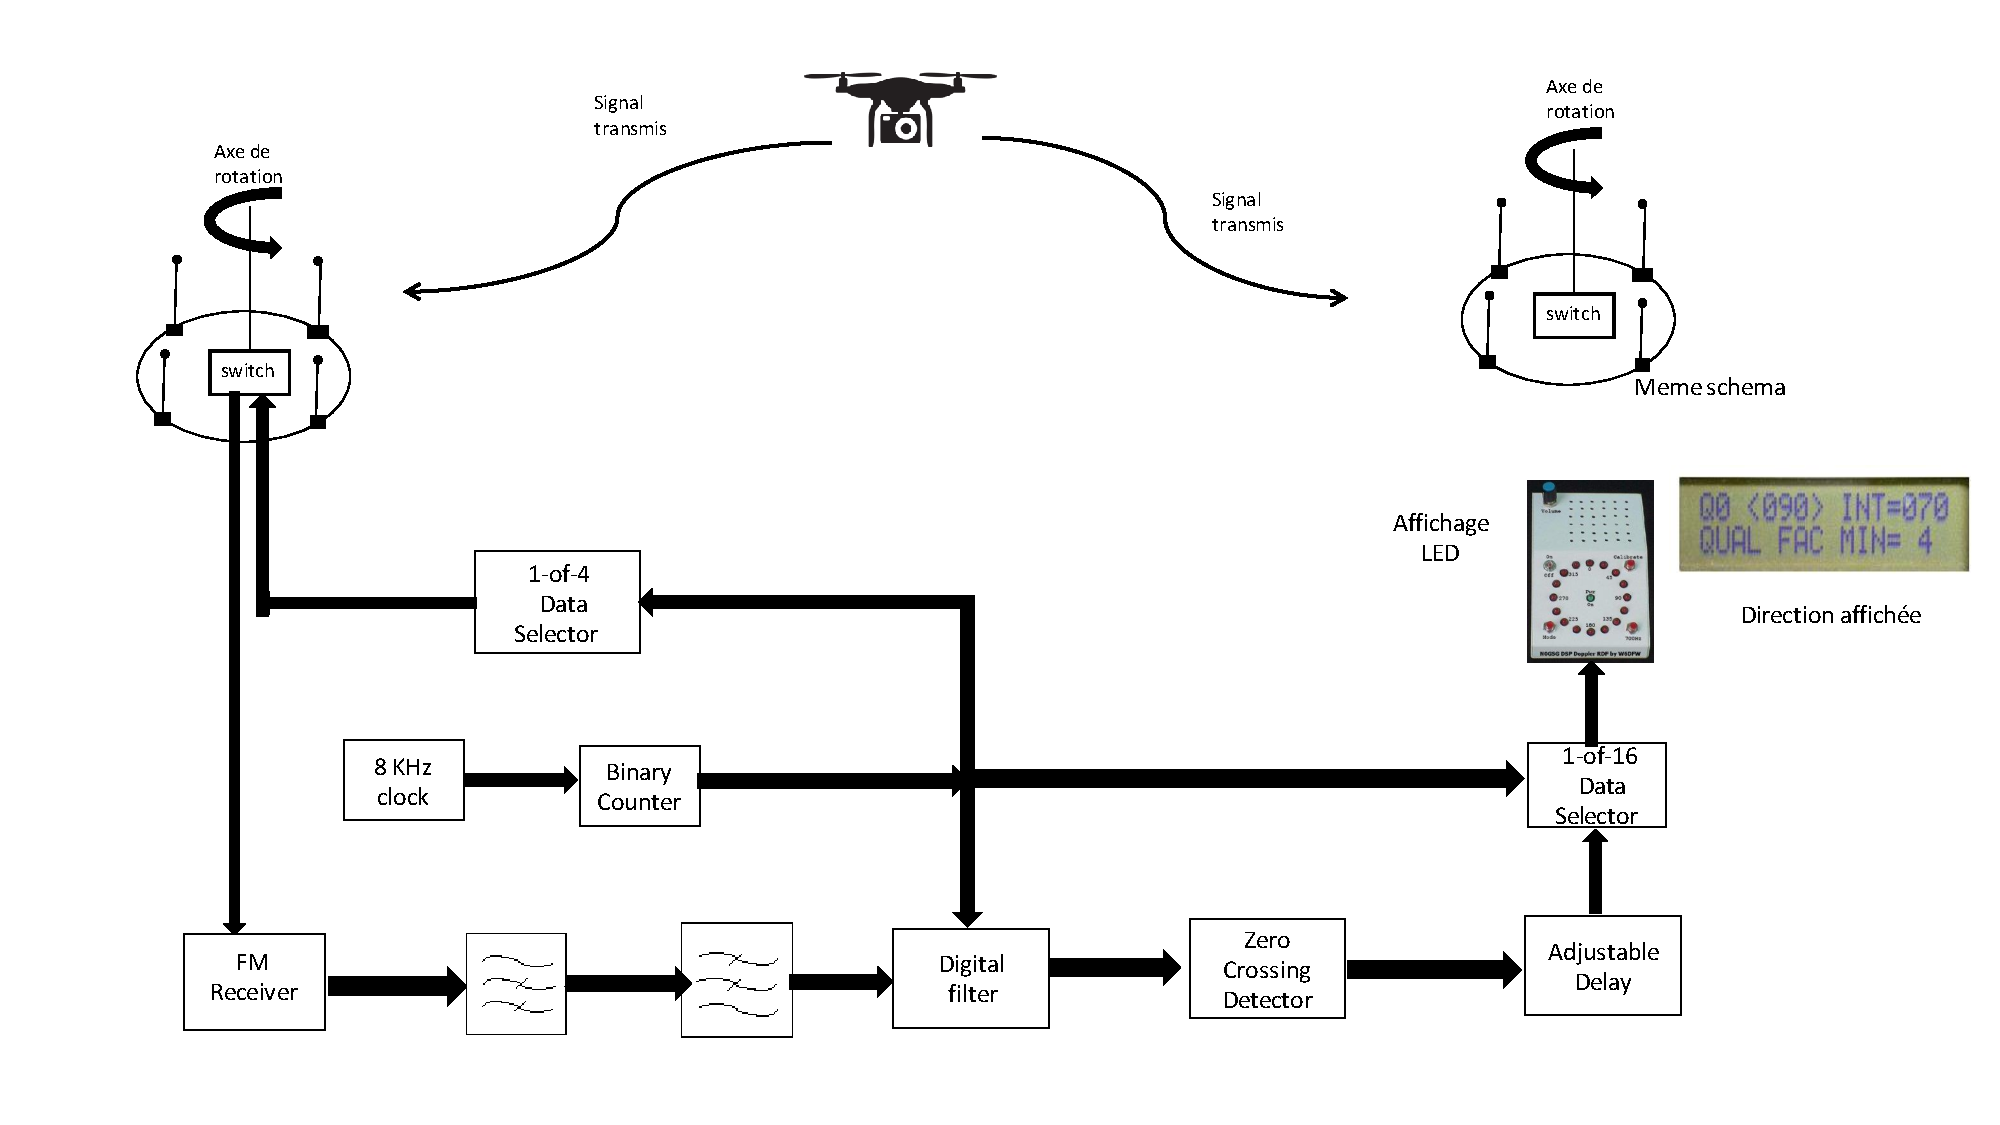
\includegraphics[width=\textwidth]{Presentation1}
\captionof{figure}{Présentation détaillée du système}
\parindent=15pt


\section{Schéma bloc}

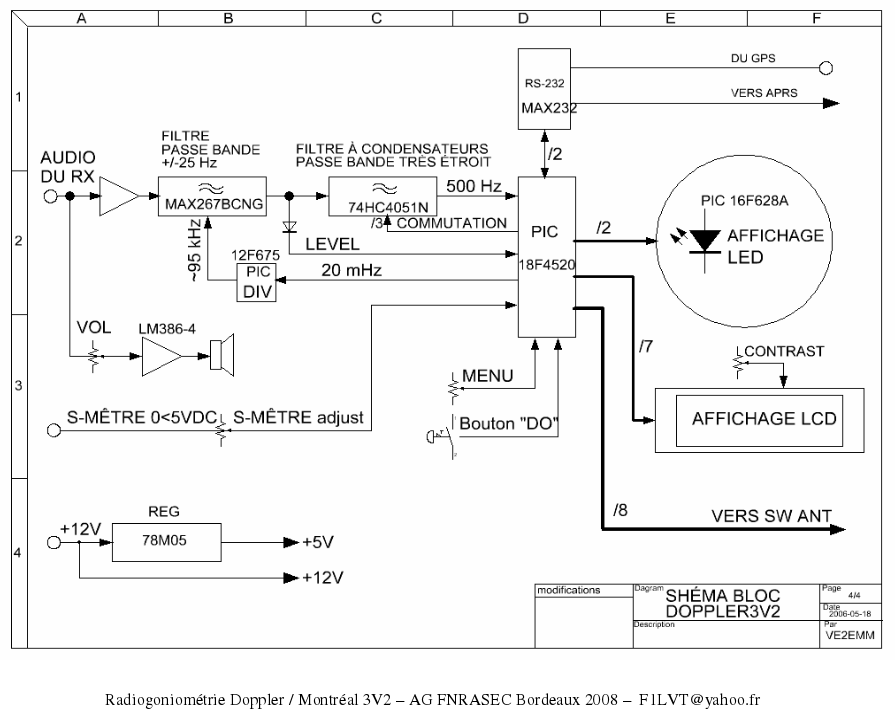
\includegraphics[width=\textwidth]{schemaBloc}
\captionof{figure}{Schéma bloc du Montréal 3v2}
\parindent=15pt

\section{Liste des composants}
Voici la liste des composants pour la construction du Montréal 3v2:

\begin{tabular}{ l l l}

IC30&          LM386N-4&                  Ampli BF\\
IC50&          MAX267BCNG&          Filtre\\
IC51& PIC  12F675-I/P& PIC \\
IC52&          74HC4051N&               Filtre\\
IC53&          MAX492CPA &            Ampli Op\\
IC70& PIC  18F4520-I/P& PIC\\
VR20 &       7805 TO-220  &            Régulateur\\
X70&           20 MHz  HC49&           Quartz\\
D50&           1N5819       &                Diode Schottky\\
LCD20&      LCD 2X16,&                 Afficheur 2 lignes de 16 car.\\
IC1& PIC16F628A-I/P& PIC\\
LED1 - LED36& ø3mm, Rouge et/ou Vert&\\
LED37&                        3 ou 5mm Bicolore Rouge/Verte &\\
FB1 - FB8&                   Ferrites\footnote{+ composants passifs : Résistances, Condensateurs.}&\\
IC100&        = MAX232ACPE&        en option\\
Q100 &        = 2N2222 TO-92&\\
\end{tabular}
\captionof{figure}{Liste des composants}
\parindent=15pt

\section{Modification à apporter}

	Le Montréal ne correspond qu'en partie à nos critères. Il est donc impératif de le modifier.
	Le premier problème concerne la gamme de fréquence du système. En effet, notre démonstrateur doit pouvoir localiser un drone émettant en 2,4 Ghz. Il faut donc à la fois modifier le bloc antenne mais également la partie de comutation d'antenne permettant de réaliser l'effet Doppler. L'étude des antennes à déjà été réalisée ci-dessus.

	De plus, pour pouvoir réaliser la localisation de la cible, il faut pouvoir réaliser le relevé de mesure en sortie du système afin d'en interpréter l'azimut de la cible par rapport au radiogoniomètre.

%%% Local Variables: 
%%% mode: latex
%%% TeX-master: "rapport_analyse"
%%% End: 
